\documentclass[]{article}
\usepackage{lmodern}
\usepackage{amssymb,amsmath}
\usepackage{ifxetex,ifluatex}
\usepackage{fixltx2e} % provides \textsubscript
\ifnum 0\ifxetex 1\fi\ifluatex 1\fi=0 % if pdftex
  \usepackage[T1]{fontenc}
  \usepackage[utf8]{inputenc}
\else % if luatex or xelatex
  \ifxetex
    \usepackage{mathspec}
  \else
    \usepackage{fontspec}
  \fi
  \defaultfontfeatures{Ligatures=TeX,Scale=MatchLowercase}
\fi
% use upquote if available, for straight quotes in verbatim environments
\IfFileExists{upquote.sty}{\usepackage{upquote}}{}
% use microtype if available
\IfFileExists{microtype.sty}{%
\usepackage{microtype}
\UseMicrotypeSet[protrusion]{basicmath} % disable protrusion for tt fonts
}{}
\usepackage[margin=1in]{geometry}
\usepackage{hyperref}
\hypersetup{unicode=true,
            pdftitle={Basic R functionality},
            pdfborder={0 0 0},
            breaklinks=true}
\urlstyle{same}  % don't use monospace font for urls
\usepackage{color}
\usepackage{fancyvrb}
\newcommand{\VerbBar}{|}
\newcommand{\VERB}{\Verb[commandchars=\\\{\}]}
\DefineVerbatimEnvironment{Highlighting}{Verbatim}{commandchars=\\\{\}}
% Add ',fontsize=\small' for more characters per line
\usepackage{framed}
\definecolor{shadecolor}{RGB}{248,248,248}
\newenvironment{Shaded}{\begin{snugshade}}{\end{snugshade}}
\newcommand{\AlertTok}[1]{\textcolor[rgb]{0.94,0.16,0.16}{#1}}
\newcommand{\AnnotationTok}[1]{\textcolor[rgb]{0.56,0.35,0.01}{\textbf{\textit{#1}}}}
\newcommand{\AttributeTok}[1]{\textcolor[rgb]{0.77,0.63,0.00}{#1}}
\newcommand{\BaseNTok}[1]{\textcolor[rgb]{0.00,0.00,0.81}{#1}}
\newcommand{\BuiltInTok}[1]{#1}
\newcommand{\CharTok}[1]{\textcolor[rgb]{0.31,0.60,0.02}{#1}}
\newcommand{\CommentTok}[1]{\textcolor[rgb]{0.56,0.35,0.01}{\textit{#1}}}
\newcommand{\CommentVarTok}[1]{\textcolor[rgb]{0.56,0.35,0.01}{\textbf{\textit{#1}}}}
\newcommand{\ConstantTok}[1]{\textcolor[rgb]{0.00,0.00,0.00}{#1}}
\newcommand{\ControlFlowTok}[1]{\textcolor[rgb]{0.13,0.29,0.53}{\textbf{#1}}}
\newcommand{\DataTypeTok}[1]{\textcolor[rgb]{0.13,0.29,0.53}{#1}}
\newcommand{\DecValTok}[1]{\textcolor[rgb]{0.00,0.00,0.81}{#1}}
\newcommand{\DocumentationTok}[1]{\textcolor[rgb]{0.56,0.35,0.01}{\textbf{\textit{#1}}}}
\newcommand{\ErrorTok}[1]{\textcolor[rgb]{0.64,0.00,0.00}{\textbf{#1}}}
\newcommand{\ExtensionTok}[1]{#1}
\newcommand{\FloatTok}[1]{\textcolor[rgb]{0.00,0.00,0.81}{#1}}
\newcommand{\FunctionTok}[1]{\textcolor[rgb]{0.00,0.00,0.00}{#1}}
\newcommand{\ImportTok}[1]{#1}
\newcommand{\InformationTok}[1]{\textcolor[rgb]{0.56,0.35,0.01}{\textbf{\textit{#1}}}}
\newcommand{\KeywordTok}[1]{\textcolor[rgb]{0.13,0.29,0.53}{\textbf{#1}}}
\newcommand{\NormalTok}[1]{#1}
\newcommand{\OperatorTok}[1]{\textcolor[rgb]{0.81,0.36,0.00}{\textbf{#1}}}
\newcommand{\OtherTok}[1]{\textcolor[rgb]{0.56,0.35,0.01}{#1}}
\newcommand{\PreprocessorTok}[1]{\textcolor[rgb]{0.56,0.35,0.01}{\textit{#1}}}
\newcommand{\RegionMarkerTok}[1]{#1}
\newcommand{\SpecialCharTok}[1]{\textcolor[rgb]{0.00,0.00,0.00}{#1}}
\newcommand{\SpecialStringTok}[1]{\textcolor[rgb]{0.31,0.60,0.02}{#1}}
\newcommand{\StringTok}[1]{\textcolor[rgb]{0.31,0.60,0.02}{#1}}
\newcommand{\VariableTok}[1]{\textcolor[rgb]{0.00,0.00,0.00}{#1}}
\newcommand{\VerbatimStringTok}[1]{\textcolor[rgb]{0.31,0.60,0.02}{#1}}
\newcommand{\WarningTok}[1]{\textcolor[rgb]{0.56,0.35,0.01}{\textbf{\textit{#1}}}}
\usepackage{graphicx,grffile}
\makeatletter
\def\maxwidth{\ifdim\Gin@nat@width>\linewidth\linewidth\else\Gin@nat@width\fi}
\def\maxheight{\ifdim\Gin@nat@height>\textheight\textheight\else\Gin@nat@height\fi}
\makeatother
% Scale images if necessary, so that they will not overflow the page
% margins by default, and it is still possible to overwrite the defaults
% using explicit options in \includegraphics[width, height, ...]{}
\setkeys{Gin}{width=\maxwidth,height=\maxheight,keepaspectratio}
\IfFileExists{parskip.sty}{%
\usepackage{parskip}
}{% else
\setlength{\parindent}{0pt}
\setlength{\parskip}{6pt plus 2pt minus 1pt}
}
\setlength{\emergencystretch}{3em}  % prevent overfull lines
\providecommand{\tightlist}{%
  \setlength{\itemsep}{0pt}\setlength{\parskip}{0pt}}
\setcounter{secnumdepth}{0}
% Redefines (sub)paragraphs to behave more like sections
\ifx\paragraph\undefined\else
\let\oldparagraph\paragraph
\renewcommand{\paragraph}[1]{\oldparagraph{#1}\mbox{}}
\fi
\ifx\subparagraph\undefined\else
\let\oldsubparagraph\subparagraph
\renewcommand{\subparagraph}[1]{\oldsubparagraph{#1}\mbox{}}
\fi

%%% Use protect on footnotes to avoid problems with footnotes in titles
\let\rmarkdownfootnote\footnote%
\def\footnote{\protect\rmarkdownfootnote}

%%% Change title format to be more compact
\usepackage{titling}

% Create subtitle command for use in maketitle
\providecommand{\subtitle}[1]{
  \posttitle{
    \begin{center}\large#1\end{center}
    }
}

\setlength{\droptitle}{-2em}

  \title{Basic R functionality}
    \pretitle{\vspace{\droptitle}\centering\huge}
  \posttitle{\par}
    \author{}
    \preauthor{}\postauthor{}
    \date{}
    \predate{}\postdate{}
  

\begin{document}
\maketitle

\hypertarget{libraries-and-setup}{%
\subsubsection{Libraries and setup}\label{libraries-and-setup}}

\begin{Shaded}
\begin{Highlighting}[]
\FunctionTok{library}\NormalTok{(readr)}
\FunctionTok{setwd}\NormalTok{(}\StringTok{"D:/Rdir/r\_for\_healthcare/basics/"}\NormalTok{)}
\end{Highlighting}
\end{Shaded}

This is an \href{http://rmarkdown.rstudio.com}{R Markdown} Notebook.
When you execute code within the notebook, the results appear beneath
the code.

Try executing this chunk by clicking the \emph{Run} button within the
chunk or by placing your cursor inside it and pressing
\emph{Ctrl+Shift+Enter}.

\begin{Shaded}
\begin{Highlighting}[]
\FunctionTok{plot}\NormalTok{(cars)}
\end{Highlighting}
\end{Shaded}

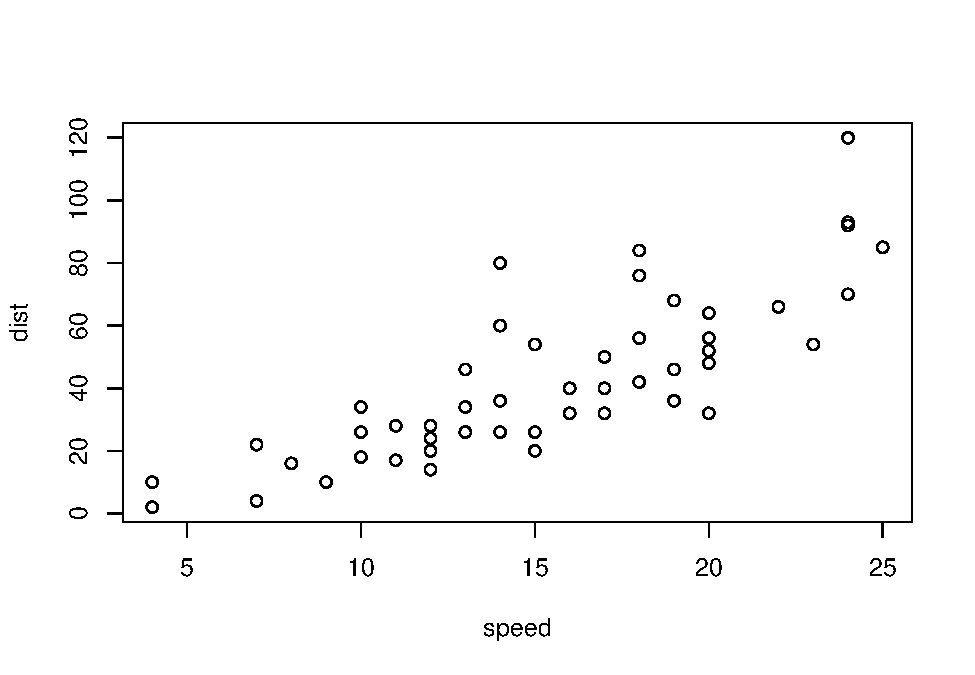
\includegraphics{basics_files/figure-latex/unnamed-chunk-2-1.pdf}

Add a new chunk by clicking the \emph{Insert Chunk} button on the
toolbar or by pressing \emph{Ctrl+Alt+I}.

When you save the notebook, an HTML file containing the code and output
will be saved alongside it (click the \emph{Preview} button or press
\emph{Ctrl+Shift+K} to preview the HTML file).

The preview shows you a rendered HTML copy of the contents of the
editor. Consequently, unlike \emph{Knit}, \emph{Preview} does not run
any R code chunks. Instead, the output of the chunk when it was last run
in the editor is displayed.

\hypertarget{readingwriting-data}{%
\subsubsection{Reading/writing data}\label{readingwriting-data}}

\begin{Shaded}
\begin{Highlighting}[]
\NormalTok{ghq }\OtherTok{\textless{}{-}} \FunctionTok{read.csv}\NormalTok{(}\StringTok{"GHQ.csv"}\NormalTok{)}
\NormalTok{ghq}
\end{Highlighting}
\end{Shaded}

\begin{verbatim}
##     X GHQ    sex cases non.cases
## 1   1   0 female     4        80
## 2   2   1 female     4        29
## 3   3   2 female     8        15
## 4   4   3 female     6         3
## 5   5   4 female     4         2
## 6   6   5 female     6         1
## 7   7   6 female     3         1
## 8   8   7 female     2         0
## 9   9   8 female     3         0
## 10 10   9 female     2         0
## 11 11  10 female     1         0
## 12 12   0   male     1        36
## 13 13   1   male     2        25
## 14 14   2   male     2         8
## 15 15   3   male     1         4
## 16 16   4   male     3         1
## 17 17   5   male     3         1
## 18 18   6   male     2         1
## 19 19   7   male     4         2
## 20 20   8   male     3         1
## 21 21   9   male     2         0
## 22 22  10   male     2         0
\end{verbatim}

\begin{Shaded}
\begin{Highlighting}[]
\FunctionTok{write.csv}\NormalTok{(ghq, }\StringTok{"GHQ2.csv"}\NormalTok{)}
\NormalTok{a}\OtherTok{\textless{}{-}}\FunctionTok{matrix}\NormalTok{(}\DecValTok{1}\SpecialCharTok{:}\DecValTok{4}\NormalTok{,}\AttributeTok{nrow=}\DecValTok{2}\NormalTok{,}\AttributeTok{ncol=}\DecValTok{2}\NormalTok{)}
\FunctionTok{write.csv}\NormalTok{(a,}\StringTok{"matrix.csv"}\NormalTok{)}
\end{Highlighting}
\end{Shaded}

\hypertarget{subscript-and-subset}{%
\subsubsection{Subscript and subset}\label{subscript-and-subset}}

\begin{Shaded}
\begin{Highlighting}[]
\NormalTok{x }\OtherTok{\textless{}{-}} \FunctionTok{seq}\NormalTok{(}\DecValTok{1}\NormalTok{,}\DecValTok{10}\NormalTok{,}\AttributeTok{by=}\FloatTok{0.5}\NormalTok{)}
\NormalTok{x[}\DecValTok{2}\NormalTok{]}
\end{Highlighting}
\end{Shaded}

\begin{verbatim}
## [1] 1.5
\end{verbatim}

\begin{Shaded}
\begin{Highlighting}[]
\NormalTok{x[}\FunctionTok{c}\NormalTok{(}\DecValTok{4}\NormalTok{,}\DecValTok{7}\NormalTok{)]}
\end{Highlighting}
\end{Shaded}

\begin{verbatim}
## [1] 2.5 4.0
\end{verbatim}

\begin{Shaded}
\begin{Highlighting}[]
\NormalTok{y }\OtherTok{\textless{}{-}} \FunctionTok{c}\NormalTok{(}\DecValTok{3}\NormalTok{,}\DecValTok{7}\NormalTok{,}\DecValTok{5}\NormalTok{,}\DecValTok{2}\NormalTok{,}\DecValTok{8}\NormalTok{)}
\NormalTok{l }\OtherTok{\textless{}{-}}\NormalTok{ y }\SpecialCharTok{\textgreater{}} \DecValTok{3}
\NormalTok{l}
\end{Highlighting}
\end{Shaded}

\begin{verbatim}
## [1] FALSE  TRUE  TRUE FALSE  TRUE
\end{verbatim}

\begin{Shaded}
\begin{Highlighting}[]
\NormalTok{y[l]}
\end{Highlighting}
\end{Shaded}

\begin{verbatim}
## [1] 7 5 8
\end{verbatim}

\begin{Shaded}
\begin{Highlighting}[]
\NormalTok{y[}\SpecialCharTok{{-}}\FunctionTok{c}\NormalTok{(}\DecValTok{2}\NormalTok{,}\DecValTok{4}\NormalTok{)]}
\end{Highlighting}
\end{Shaded}

\begin{verbatim}
## [1] 3 5 8
\end{verbatim}

\begin{Shaded}
\begin{Highlighting}[]
\NormalTok{z }\OtherTok{\textless{}{-}} \FunctionTok{matrix}\NormalTok{(}\FunctionTok{c}\NormalTok{(}\DecValTok{1}\NormalTok{,}\DecValTok{2}\NormalTok{,}\DecValTok{5}\NormalTok{,}\DecValTok{3}\NormalTok{,}\DecValTok{2}\NormalTok{,}\DecValTok{4}\NormalTok{,}\DecValTok{6}\NormalTok{,}\DecValTok{4}\NormalTok{,}\DecValTok{5}\NormalTok{,}\DecValTok{3}\NormalTok{,}\DecValTok{6}\NormalTok{,}\DecValTok{1}\NormalTok{), }\AttributeTok{nrow=}\DecValTok{3}\NormalTok{, }\AttributeTok{ncol=}\DecValTok{4}\NormalTok{, }\AttributeTok{byrow=}\ConstantTok{TRUE}\NormalTok{)}
\FunctionTok{print}\NormalTok{(z)}
\end{Highlighting}
\end{Shaded}

\begin{verbatim}
##      [,1] [,2] [,3] [,4]
## [1,]    1    2    5    3
## [2,]    2    4    6    4
## [3,]    5    3    6    1
\end{verbatim}

\begin{Shaded}
\begin{Highlighting}[]
\NormalTok{z[}\DecValTok{2}\NormalTok{,]}
\end{Highlighting}
\end{Shaded}

\begin{verbatim}
## [1] 2 4 6 4
\end{verbatim}

\begin{Shaded}
\begin{Highlighting}[]
\NormalTok{z[,}\DecValTok{4}\NormalTok{]}
\end{Highlighting}
\end{Shaded}

\begin{verbatim}
## [1] 3 4 1
\end{verbatim}

\begin{Shaded}
\begin{Highlighting}[]
\NormalTok{z[}\DecValTok{2}\NormalTok{,}\DecValTok{4}\NormalTok{]}
\end{Highlighting}
\end{Shaded}

\begin{verbatim}
## [1] 4
\end{verbatim}

\begin{Shaded}
\begin{Highlighting}[]
\NormalTok{z[}\FunctionTok{c}\NormalTok{(}\DecValTok{1}\NormalTok{,}\DecValTok{2}\NormalTok{),]}
\end{Highlighting}
\end{Shaded}

\begin{verbatim}
##      [,1] [,2] [,3] [,4]
## [1,]    1    2    5    3
## [2,]    2    4    6    4
\end{verbatim}

\begin{Shaded}
\begin{Highlighting}[]
\NormalTok{z[,}\FunctionTok{c}\NormalTok{(}\DecValTok{1}\NormalTok{,}\DecValTok{2}\NormalTok{)]}
\end{Highlighting}
\end{Shaded}

\begin{verbatim}
##      [,1] [,2]
## [1,]    1    2
## [2,]    2    4
## [3,]    5    3
\end{verbatim}

\begin{Shaded}
\begin{Highlighting}[]
\NormalTok{z[}\FunctionTok{c}\NormalTok{(T,F,T),]}
\end{Highlighting}
\end{Shaded}

\begin{verbatim}
##      [,1] [,2] [,3] [,4]
## [1,]    1    2    5    3
## [2,]    5    3    6    1
\end{verbatim}

\begin{Shaded}
\begin{Highlighting}[]
\NormalTok{data }\OtherTok{\textless{}{-}} \FunctionTok{as.data.frame}\NormalTok{(z)}
\NormalTok{data}
\end{Highlighting}
\end{Shaded}

\begin{verbatim}
##   V1 V2 V3 V4
## 1  1  2  5  3
## 2  2  4  6  4
## 3  5  3  6  1
\end{verbatim}

\begin{Shaded}
\begin{Highlighting}[]
\NormalTok{dataOne }\OtherTok{\textless{}{-}}\NormalTok{ data}\SpecialCharTok{$}\NormalTok{V1}
\NormalTok{dataOne}
\end{Highlighting}
\end{Shaded}

\begin{verbatim}
## [1] 1 2 5
\end{verbatim}

\begin{Shaded}
\begin{Highlighting}[]
\FunctionTok{attach}\NormalTok{(data)}
\NormalTok{dataOne }\OtherTok{\textless{}{-}}\NormalTok{ V1}
\NormalTok{dataOne}
\end{Highlighting}
\end{Shaded}

\begin{verbatim}
## [1] 1 2 5
\end{verbatim}

\begin{Shaded}
\begin{Highlighting}[]
\FunctionTok{detach}\NormalTok{(data)}
\NormalTok{dataOne }\OtherTok{\textless{}{-}}\NormalTok{ data[}\FunctionTok{c}\NormalTok{(}\StringTok{"V2"}\NormalTok{, }\StringTok{"V3"}\NormalTok{)]}
\NormalTok{dataOne}
\end{Highlighting}
\end{Shaded}

\begin{verbatim}
##   V2 V3
## 1  2  5
## 2  4  6
## 3  3  6
\end{verbatim}

\begin{Shaded}
\begin{Highlighting}[]
\NormalTok{dataTwo }\OtherTok{\textless{}{-}}\NormalTok{ data[}\DecValTok{1}\SpecialCharTok{:}\DecValTok{2}\NormalTok{, ]}
\end{Highlighting}
\end{Shaded}

\begin{Shaded}
\begin{Highlighting}[]
\NormalTok{dataFour }\OtherTok{\textless{}{-}}\NormalTok{ data[}\FunctionTok{which}\NormalTok{(data}\SpecialCharTok{$}\NormalTok{V1 }\SpecialCharTok{==} \DecValTok{2} \SpecialCharTok{|}\NormalTok{ data}\SpecialCharTok{$}\NormalTok{V3 }\SpecialCharTok{==} \DecValTok{6}\NormalTok{), ]}
\NormalTok{dataFour}
\end{Highlighting}
\end{Shaded}

\begin{verbatim}
##   V1 V2 V3 V4
## 2  2  4  6  4
## 3  5  3  6  1
\end{verbatim}

\hypertarget{merge-and-append-data}{%
\subsubsection{Merge and append data}\label{merge-and-append-data}}

\begin{Shaded}
\begin{Highlighting}[]
\NormalTok{A }\OtherTok{\textless{}{-}} \FunctionTok{matrix}\NormalTok{(}\FunctionTok{c}\NormalTok{(}\DecValTok{1}\NormalTok{,}\DecValTok{2}\NormalTok{,}\DecValTok{3}\NormalTok{,}\DecValTok{4}\NormalTok{), }\AttributeTok{nrow=}\DecValTok{2}\NormalTok{, }\AttributeTok{ncol=}\DecValTok{2}\NormalTok{)}
\NormalTok{A}
\end{Highlighting}
\end{Shaded}

\begin{verbatim}
##      [,1] [,2]
## [1,]    1    3
## [2,]    2    4
\end{verbatim}

\begin{Shaded}
\begin{Highlighting}[]
\NormalTok{B }\OtherTok{\textless{}{-}} \FunctionTok{c}\NormalTok{(}\DecValTok{5}\NormalTok{,}\DecValTok{6}\NormalTok{)}
\NormalTok{C }\OtherTok{\textless{}{-}} \FunctionTok{rbind}\NormalTok{(A,B)}
\NormalTok{C}
\end{Highlighting}
\end{Shaded}

\begin{verbatim}
##   [,1] [,2]
##      1    3
##      2    4
## B    5    6
\end{verbatim}

\begin{Shaded}
\begin{Highlighting}[]
\NormalTok{D }\OtherTok{\textless{}{-}} \FunctionTok{c}\NormalTok{(}\DecValTok{5}\NormalTok{,}\DecValTok{6}\NormalTok{)}
\NormalTok{E }\OtherTok{\textless{}{-}} \FunctionTok{cbind}\NormalTok{(A,D)}
\NormalTok{E}
\end{Highlighting}
\end{Shaded}

\begin{verbatim}
##          D
## [1,] 1 3 5
## [2,] 2 4 6
\end{verbatim}

\begin{Shaded}
\begin{Highlighting}[]
\NormalTok{a }\OtherTok{\textless{}{-}} \FunctionTok{c}\NormalTok{(}\DecValTok{1}\NormalTok{,}\DecValTok{2}\NormalTok{,}\DecValTok{3}\NormalTok{,}\DecValTok{4}\NormalTok{)}
\NormalTok{b }\OtherTok{\textless{}{-}} \FunctionTok{append}\NormalTok{(a,}\FunctionTok{c}\NormalTok{(}\DecValTok{5}\NormalTok{,}\DecValTok{6}\NormalTok{))}
\NormalTok{b}
\end{Highlighting}
\end{Shaded}

\begin{verbatim}
## [1] 1 2 3 4 5 6
\end{verbatim}

\begin{Shaded}
\begin{Highlighting}[]
\NormalTok{a }\OtherTok{\textless{}{-}} \FunctionTok{c}\NormalTok{(}\DecValTok{1}\NormalTok{,}\DecValTok{2}\NormalTok{,}\DecValTok{3}\NormalTok{,}\DecValTok{4}\NormalTok{)}
\NormalTok{b }\OtherTok{\textless{}{-}} \FunctionTok{append}\NormalTok{(a,}\FunctionTok{c}\NormalTok{(}\DecValTok{5}\NormalTok{,}\DecValTok{6}\NormalTok{), }\AttributeTok{after=}\DecValTok{2}\NormalTok{)}
\NormalTok{b}
\end{Highlighting}
\end{Shaded}

\begin{verbatim}
## [1] 1 2 5 6 3 4
\end{verbatim}

\begin{Shaded}
\begin{Highlighting}[]
\NormalTok{clinical\_trial1 }\OtherTok{\textless{}{-}} \FunctionTok{data.frame}\NormalTok{(}\AttributeTok{patient=}\DecValTok{1}\SpecialCharTok{:}\DecValTok{100}\NormalTok{,}
                              \AttributeTok{age=}\FunctionTok{signif}\NormalTok{(}\FunctionTok{rnorm}\NormalTok{(}\DecValTok{100}\NormalTok{, }\AttributeTok{mean=}\DecValTok{60}\NormalTok{, }\AttributeTok{sd=}\DecValTok{6}\NormalTok{),}
                                         \AttributeTok{digits=}\DecValTok{2}\NormalTok{),}
                              \AttributeTok{treatment =} \FunctionTok{gl}\NormalTok{(}\DecValTok{2}\NormalTok{,}\DecValTok{50}\NormalTok{,}\AttributeTok{labels=}\FunctionTok{c}\NormalTok{(}\StringTok{"Treatment"}\NormalTok{, }\StringTok{"Control"}\NormalTok{)),}
                              \AttributeTok{centre =} \FunctionTok{sample}\NormalTok{(}\FunctionTok{paste}\NormalTok{(}\StringTok{"Centre"}\NormalTok{, LETTERS[}\DecValTok{1}\SpecialCharTok{:}\DecValTok{5}\NormalTok{]),}
                                                          \DecValTok{100}\NormalTok{, }\AttributeTok{replace=}\ConstantTok{TRUE}\NormalTok{))}
\NormalTok{clinical\_trial1}
\end{Highlighting}
\end{Shaded}

\begin{verbatim}
##     patient age treatment   centre
## 1         1  60 Treatment Centre A
## 2         2  64 Treatment Centre D
## 3         3  56 Treatment Centre C
## 4         4  65 Treatment Centre E
## 5         5  66 Treatment Centre A
## 6         6  62 Treatment Centre C
## 7         7  63 Treatment Centre C
## 8         8  58 Treatment Centre B
## 9         9  62 Treatment Centre D
## 10       10  64 Treatment Centre C
## 11       11  61 Treatment Centre D
## 12       12  46 Treatment Centre C
## 13       13  58 Treatment Centre D
## 14       14  68 Treatment Centre E
## 15       15  56 Treatment Centre C
## 16       16  68 Treatment Centre E
## 17       17  56 Treatment Centre B
## 18       18  59 Treatment Centre A
## 19       19  57 Treatment Centre A
## 20       20  57 Treatment Centre D
## 21       21  67 Treatment Centre E
## 22       22  68 Treatment Centre C
## 23       23  58 Treatment Centre C
## 24       24  63 Treatment Centre B
## 25       25  66 Treatment Centre D
## 26       26  54 Treatment Centre D
## 27       27  56 Treatment Centre B
## 28       28  61 Treatment Centre C
## 29       29  53 Treatment Centre E
## 30       30  65 Treatment Centre E
## 31       31  64 Treatment Centre A
## 32       32  58 Treatment Centre B
## 33       33  56 Treatment Centre C
## 34       34  62 Treatment Centre C
## 35       35  47 Treatment Centre B
## 36       36  62 Treatment Centre A
## 37       37  52 Treatment Centre D
## 38       38  58 Treatment Centre B
## 39       39  63 Treatment Centre B
## 40       40  51 Treatment Centre C
## 41       41  48 Treatment Centre E
## 42       42  62 Treatment Centre E
## 43       43  61 Treatment Centre A
## 44       44  64 Treatment Centre C
## 45       45  70 Treatment Centre A
## 46       46  61 Treatment Centre E
## 47       47  55 Treatment Centre D
## 48       48  58 Treatment Centre B
## 49       49  46 Treatment Centre E
## 50       50  55 Treatment Centre A
## 51       51  62   Control Centre D
## 52       52  60   Control Centre A
## 53       53  64   Control Centre A
## 54       54  61   Control Centre D
## 55       55  62   Control Centre E
## 56       56  67   Control Centre B
## 57       57  57   Control Centre A
## 58       58  62   Control Centre E
## 59       59  53   Control Centre C
## 60       60  64   Control Centre B
## 61       61  62   Control Centre C
## 62       62  73   Control Centre A
## 63       63  69   Control Centre B
## 64       64  70   Control Centre C
## 65       65  47   Control Centre B
## 66       66  61   Control Centre D
## 67       67  57   Control Centre C
## 68       68  71   Control Centre B
## 69       69  67   Control Centre E
## 70       70  64   Control Centre D
## 71       71  66   Control Centre D
## 72       72  56   Control Centre E
## 73       73  62   Control Centre E
## 74       74  63   Control Centre E
## 75       75  60   Control Centre B
## 76       76  65   Control Centre E
## 77       77  55   Control Centre D
## 78       78  64   Control Centre B
## 79       79  59   Control Centre E
## 80       80  78   Control Centre C
## 81       81  58   Control Centre E
## 82       82  59   Control Centre E
## 83       83  61   Control Centre B
## 84       84  55   Control Centre C
## 85       85  53   Control Centre C
## 86       86  79   Control Centre B
## 87       87  62   Control Centre B
## 88       88  53   Control Centre A
## 89       89  57   Control Centre E
## 90       90  59   Control Centre D
## 91       91  63   Control Centre A
## 92       92  50   Control Centre A
## 93       93  61   Control Centre D
## 94       94  54   Control Centre A
## 95       95  61   Control Centre E
## 96       96  55   Control Centre E
## 97       97  64   Control Centre D
## 98       98  59   Control Centre C
## 99       99  62   Control Centre B
## 100     100  58   Control Centre A
\end{verbatim}

\begin{Shaded}
\begin{Highlighting}[]
\NormalTok{clinical\_trial2 }\OtherTok{\textless{}{-}} \FunctionTok{data.frame}\NormalTok{(}\AttributeTok{patient =} \DecValTok{1}\SpecialCharTok{:}\DecValTok{100}\NormalTok{,}
                              \AttributeTok{BMI =} \FunctionTok{rpois}\NormalTok{(}\DecValTok{100}\NormalTok{, }\AttributeTok{lambda=}\DecValTok{25}\NormalTok{),}
                              \AttributeTok{gender =} \FunctionTok{rep}\NormalTok{(}\FunctionTok{gl}\NormalTok{(}\DecValTok{2}\NormalTok{,}\DecValTok{25}\NormalTok{,}\AttributeTok{labels=}\FunctionTok{c}\NormalTok{(}\StringTok{"Male"}\NormalTok{, }\StringTok{"Female"}\NormalTok{),}\AttributeTok{ordered=}\ConstantTok{FALSE}\NormalTok{),}
                                           \AttributeTok{times=}\DecValTok{2}\NormalTok{))}
\NormalTok{clinical\_trial2}
\end{Highlighting}
\end{Shaded}

\begin{verbatim}
##     patient BMI gender
## 1         1  17   Male
## 2         2  22   Male
## 3         3  17   Male
## 4         4  18   Male
## 5         5  30   Male
## 6         6  31   Male
## 7         7  28   Male
## 8         8  25   Male
## 9         9  22   Male
## 10       10  24   Male
## 11       11  29   Male
## 12       12  22   Male
## 13       13  18   Male
## 14       14  22   Male
## 15       15  31   Male
## 16       16  23   Male
## 17       17  33   Male
## 18       18  29   Male
## 19       19  32   Male
## 20       20  28   Male
## 21       21  23   Male
## 22       22  18   Male
## 23       23  15   Male
## 24       24  21   Male
## 25       25  18   Male
## 26       26  26 Female
## 27       27  28 Female
## 28       28  26 Female
## 29       29  25 Female
## 30       30  28 Female
## 31       31  21 Female
## 32       32  27 Female
## 33       33  18 Female
## 34       34  27 Female
## 35       35  34 Female
## 36       36  18 Female
## 37       37  30 Female
## 38       38  27 Female
## 39       39  19 Female
## 40       40  28 Female
## 41       41  23 Female
## 42       42  31 Female
## 43       43  26 Female
## 44       44  26 Female
## 45       45  34 Female
## 46       46  23 Female
## 47       47  31 Female
## 48       48  31 Female
## 49       49  19 Female
## 50       50  26 Female
## 51       51  24   Male
## 52       52  24   Male
## 53       53  26   Male
## 54       54  16   Male
## 55       55  20   Male
## 56       56  30   Male
## 57       57  27   Male
## 58       58  22   Male
## 59       59  22   Male
## 60       60  23   Male
## 61       61  22   Male
## 62       62  22   Male
## 63       63  22   Male
## 64       64  26   Male
## 65       65  29   Male
## 66       66  26   Male
## 67       67  22   Male
## 68       68  21   Male
## 69       69  21   Male
## 70       70  24   Male
## 71       71  25   Male
## 72       72  32   Male
## 73       73  14   Male
## 74       74  25   Male
## 75       75  25   Male
## 76       76  22 Female
## 77       77  24 Female
## 78       78  20 Female
## 79       79  33 Female
## 80       80  26 Female
## 81       81  21 Female
## 82       82  25 Female
## 83       83  20 Female
## 84       84  38 Female
## 85       85  16 Female
## 86       86  27 Female
## 87       87  28 Female
## 88       88  24 Female
## 89       89  24 Female
## 90       90  33 Female
## 91       91  26 Female
## 92       92  20 Female
## 93       93  30 Female
## 94       94  24 Female
## 95       95  24 Female
## 96       96  18 Female
## 97       97  25 Female
## 98       98  20 Female
## 99       99  25 Female
## 100     100  21 Female
\end{verbatim}

\begin{Shaded}
\begin{Highlighting}[]
\NormalTok{clinical\_trial3 }\OtherTok{\textless{}{-}} \FunctionTok{merge}\NormalTok{(clinical\_trial1, clinical\_trial2, }\AttributeTok{by.x=}\StringTok{\textquotesingle{}patient\textquotesingle{}}\NormalTok{, }\AttributeTok{by.y=}\StringTok{\textquotesingle{}patient\textquotesingle{}}\NormalTok{,}
                         \AttributeTok{all=}\ConstantTok{TRUE}\NormalTok{)}
\NormalTok{clinical\_trial3[}\DecValTok{1}\SpecialCharTok{:}\DecValTok{10}\NormalTok{,]}
\end{Highlighting}
\end{Shaded}

\begin{verbatim}
##    patient age treatment   centre BMI gender
## 1        1  60 Treatment Centre A  17   Male
## 2        2  64 Treatment Centre D  22   Male
## 3        3  56 Treatment Centre C  17   Male
## 4        4  65 Treatment Centre E  18   Male
## 5        5  66 Treatment Centre A  30   Male
## 6        6  62 Treatment Centre C  31   Male
## 7        7  63 Treatment Centre C  28   Male
## 8        8  58 Treatment Centre B  25   Male
## 9        9  62 Treatment Centre D  22   Male
## 10      10  64 Treatment Centre C  24   Male
\end{verbatim}

\begin{Shaded}
\begin{Highlighting}[]
\NormalTok{GP }\OtherTok{\textless{}{-}} \FunctionTok{rep}\NormalTok{(}\DecValTok{1}\SpecialCharTok{:}\DecValTok{5}\NormalTok{, }\DecValTok{20}\NormalTok{)}
\NormalTok{clinical\_trial4 }\OtherTok{\textless{}{-}} \FunctionTok{cbind}\NormalTok{(clinical\_trial3, GP)}
\NormalTok{clinical\_trial4}
\end{Highlighting}
\end{Shaded}

\begin{verbatim}
##     patient age treatment   centre BMI gender GP
## 1         1  60 Treatment Centre A  17   Male  1
## 2         2  64 Treatment Centre D  22   Male  2
## 3         3  56 Treatment Centre C  17   Male  3
## 4         4  65 Treatment Centre E  18   Male  4
## 5         5  66 Treatment Centre A  30   Male  5
## 6         6  62 Treatment Centre C  31   Male  1
## 7         7  63 Treatment Centre C  28   Male  2
## 8         8  58 Treatment Centre B  25   Male  3
## 9         9  62 Treatment Centre D  22   Male  4
## 10       10  64 Treatment Centre C  24   Male  5
## 11       11  61 Treatment Centre D  29   Male  1
## 12       12  46 Treatment Centre C  22   Male  2
## 13       13  58 Treatment Centre D  18   Male  3
## 14       14  68 Treatment Centre E  22   Male  4
## 15       15  56 Treatment Centre C  31   Male  5
## 16       16  68 Treatment Centre E  23   Male  1
## 17       17  56 Treatment Centre B  33   Male  2
## 18       18  59 Treatment Centre A  29   Male  3
## 19       19  57 Treatment Centre A  32   Male  4
## 20       20  57 Treatment Centre D  28   Male  5
## 21       21  67 Treatment Centre E  23   Male  1
## 22       22  68 Treatment Centre C  18   Male  2
## 23       23  58 Treatment Centre C  15   Male  3
## 24       24  63 Treatment Centre B  21   Male  4
## 25       25  66 Treatment Centre D  18   Male  5
## 26       26  54 Treatment Centre D  26 Female  1
## 27       27  56 Treatment Centre B  28 Female  2
## 28       28  61 Treatment Centre C  26 Female  3
## 29       29  53 Treatment Centre E  25 Female  4
## 30       30  65 Treatment Centre E  28 Female  5
## 31       31  64 Treatment Centre A  21 Female  1
## 32       32  58 Treatment Centre B  27 Female  2
## 33       33  56 Treatment Centre C  18 Female  3
## 34       34  62 Treatment Centre C  27 Female  4
## 35       35  47 Treatment Centre B  34 Female  5
## 36       36  62 Treatment Centre A  18 Female  1
## 37       37  52 Treatment Centre D  30 Female  2
## 38       38  58 Treatment Centre B  27 Female  3
## 39       39  63 Treatment Centre B  19 Female  4
## 40       40  51 Treatment Centre C  28 Female  5
## 41       41  48 Treatment Centre E  23 Female  1
## 42       42  62 Treatment Centre E  31 Female  2
## 43       43  61 Treatment Centre A  26 Female  3
## 44       44  64 Treatment Centre C  26 Female  4
## 45       45  70 Treatment Centre A  34 Female  5
## 46       46  61 Treatment Centre E  23 Female  1
## 47       47  55 Treatment Centre D  31 Female  2
## 48       48  58 Treatment Centre B  31 Female  3
## 49       49  46 Treatment Centre E  19 Female  4
## 50       50  55 Treatment Centre A  26 Female  5
## 51       51  62   Control Centre D  24   Male  1
## 52       52  60   Control Centre A  24   Male  2
## 53       53  64   Control Centre A  26   Male  3
## 54       54  61   Control Centre D  16   Male  4
## 55       55  62   Control Centre E  20   Male  5
## 56       56  67   Control Centre B  30   Male  1
## 57       57  57   Control Centre A  27   Male  2
## 58       58  62   Control Centre E  22   Male  3
## 59       59  53   Control Centre C  22   Male  4
## 60       60  64   Control Centre B  23   Male  5
## 61       61  62   Control Centre C  22   Male  1
## 62       62  73   Control Centre A  22   Male  2
## 63       63  69   Control Centre B  22   Male  3
## 64       64  70   Control Centre C  26   Male  4
## 65       65  47   Control Centre B  29   Male  5
## 66       66  61   Control Centre D  26   Male  1
## 67       67  57   Control Centre C  22   Male  2
## 68       68  71   Control Centre B  21   Male  3
## 69       69  67   Control Centre E  21   Male  4
## 70       70  64   Control Centre D  24   Male  5
## 71       71  66   Control Centre D  25   Male  1
## 72       72  56   Control Centre E  32   Male  2
## 73       73  62   Control Centre E  14   Male  3
## 74       74  63   Control Centre E  25   Male  4
## 75       75  60   Control Centre B  25   Male  5
## 76       76  65   Control Centre E  22 Female  1
## 77       77  55   Control Centre D  24 Female  2
## 78       78  64   Control Centre B  20 Female  3
## 79       79  59   Control Centre E  33 Female  4
## 80       80  78   Control Centre C  26 Female  5
## 81       81  58   Control Centre E  21 Female  1
## 82       82  59   Control Centre E  25 Female  2
## 83       83  61   Control Centre B  20 Female  3
## 84       84  55   Control Centre C  38 Female  4
## 85       85  53   Control Centre C  16 Female  5
## 86       86  79   Control Centre B  27 Female  1
## 87       87  62   Control Centre B  28 Female  2
## 88       88  53   Control Centre A  24 Female  3
## 89       89  57   Control Centre E  24 Female  4
## 90       90  59   Control Centre D  33 Female  5
## 91       91  63   Control Centre A  26 Female  1
## 92       92  50   Control Centre A  20 Female  2
## 93       93  61   Control Centre D  30 Female  3
## 94       94  54   Control Centre A  24 Female  4
## 95       95  61   Control Centre E  24 Female  5
## 96       96  55   Control Centre E  18 Female  1
## 97       97  64   Control Centre D  25 Female  2
## 98       98  59   Control Centre C  20 Female  3
## 99       99  62   Control Centre B  25 Female  4
## 100     100  58   Control Centre A  21 Female  5
\end{verbatim}

\begin{Shaded}
\begin{Highlighting}[]
\NormalTok{row }\OtherTok{\textless{}{-}} \FunctionTok{c}\NormalTok{(}\DecValTok{101}\NormalTok{,}\DecValTok{57}\NormalTok{, }\StringTok{"Treatment"}\NormalTok{, }\StringTok{"Centre D"}\NormalTok{, }\DecValTok{26}\NormalTok{, }\StringTok{"Male"}\NormalTok{, }\DecValTok{4}\NormalTok{)}
\NormalTok{clinical\_trial5 }\OtherTok{\textless{}{-}} \FunctionTok{rbind}\NormalTok{(clinical\_trial4, row)}
\NormalTok{clinical\_trial5[}\DecValTok{91}\SpecialCharTok{:}\DecValTok{101}\NormalTok{,]}
\end{Highlighting}
\end{Shaded}

\begin{verbatim}
##     patient age treatment   centre BMI gender GP
## 91       91  63   Control Centre A  26 Female  1
## 92       92  50   Control Centre A  20 Female  2
## 93       93  61   Control Centre D  30 Female  3
## 94       94  54   Control Centre A  24 Female  4
## 95       95  61   Control Centre E  24 Female  5
## 96       96  55   Control Centre E  18 Female  1
## 97       97  64   Control Centre D  25 Female  2
## 98       98  59   Control Centre C  20 Female  3
## 99       99  62   Control Centre B  25 Female  4
## 100     100  58   Control Centre A  21 Female  5
## 101     101  57 Treatment Centre D  26   Male  4
\end{verbatim}

\hypertarget{sorting-data}{%
\subsubsection{Sorting data}\label{sorting-data}}

\begin{Shaded}
\begin{Highlighting}[]
\FunctionTok{data}\NormalTok{(USArrests)}
\FunctionTok{attach}\NormalTok{(USArrests)}
\NormalTok{USArrests[}\DecValTok{1}\SpecialCharTok{:}\DecValTok{10}\NormalTok{,]}
\end{Highlighting}
\end{Shaded}

\begin{verbatim}
##             Murder Assault UrbanPop Rape
## Alabama       13.2     236       58 21.2
## Alaska        10.0     263       48 44.5
## Arizona        8.1     294       80 31.0
## Arkansas       8.8     190       50 19.5
## California     9.0     276       91 40.6
## Colorado       7.9     204       78 38.7
## Connecticut    3.3     110       77 11.1
## Delaware       5.9     238       72 15.8
## Florida       15.4     335       80 31.9
## Georgia       17.4     211       60 25.8
\end{verbatim}

\begin{Shaded}
\begin{Highlighting}[]
\FunctionTok{sort}\NormalTok{(UrbanPop)}
\end{Highlighting}
\end{Shaded}

\begin{verbatim}
##  [1] 32 39 44 44 45 45 48 48 50 51 52 53 54 56 57 58 59 60 60 62 63 65 66
## [24] 66 66 66 67 67 68 70 70 72 72 73 74 75 77 78 80 80 80 80 81 83 83 85
## [47] 86 87 89 91
\end{verbatim}

\begin{Shaded}
\begin{Highlighting}[]
\NormalTok{sort1\_USarr }\OtherTok{\textless{}{-}}\NormalTok{ USArrests[}\FunctionTok{order}\NormalTok{(UrbanPop,Murder),]}
\NormalTok{sort1\_USarr[}\DecValTok{1}\SpecialCharTok{:}\DecValTok{15}\NormalTok{,]}
\end{Highlighting}
\end{Shaded}

\begin{verbatim}
##                Murder Assault UrbanPop Rape
## Vermont           2.2      48       32 11.2
## West Virginia     5.7      81       39  9.3
## North Dakota      0.8      45       44  7.3
## Mississippi      16.1     259       44 17.1
## South Dakota      3.8      86       45 12.8
## North Carolina   13.0     337       45 16.1
## Alaska           10.0     263       48 44.5
## South Carolina   14.4     279       48 22.5
## Arkansas          8.8     190       50 19.5
## Maine             2.1      83       51  7.8
## Kentucky          9.7     109       52 16.3
## Montana           6.0     109       53 16.4
## Idaho             2.6     120       54 14.2
## New Hampshire     2.1      57       56  9.5
## Iowa              2.2      56       57 11.3
\end{verbatim}

\begin{Shaded}
\begin{Highlighting}[]
\NormalTok{sort2\_USarr }\OtherTok{\textless{}{-}}\NormalTok{ USArrests[}\FunctionTok{order}\NormalTok{(UrbanPop, }\SpecialCharTok{{-}}\NormalTok{Murder),]}
\NormalTok{sort2\_USarr[}\DecValTok{1}\SpecialCharTok{:}\DecValTok{15}\NormalTok{,]}
\end{Highlighting}
\end{Shaded}

\begin{verbatim}
##                Murder Assault UrbanPop Rape
## Vermont           2.2      48       32 11.2
## West Virginia     5.7      81       39  9.3
## Mississippi      16.1     259       44 17.1
## North Dakota      0.8      45       44  7.3
## North Carolina   13.0     337       45 16.1
## South Dakota      3.8      86       45 12.8
## South Carolina   14.4     279       48 22.5
## Alaska           10.0     263       48 44.5
## Arkansas          8.8     190       50 19.5
## Maine             2.1      83       51  7.8
## Kentucky          9.7     109       52 16.3
## Montana           6.0     109       53 16.4
## Idaho             2.6     120       54 14.2
## New Hampshire     2.1      57       56  9.5
## Iowa              2.2      56       57 11.3
\end{verbatim}

\hypertarget{working-with-timedate}{%
\subsubsection{Working with time/date}\label{working-with-timedate}}

\begin{Shaded}
\begin{Highlighting}[]
\NormalTok{df\_birth }\OtherTok{\textless{}{-}} \FunctionTok{data.frame}\NormalTok{(}\AttributeTok{ID=}\DecValTok{1}\SpecialCharTok{:}\DecValTok{10}\NormalTok{,}\AttributeTok{dob=}\FunctionTok{c}\NormalTok{(}\StringTok{"12/04/1976"}\NormalTok{,}\StringTok{"16/06/1965"}\NormalTok{,}\StringTok{"23/11/1985"}\NormalTok{,}
                      \StringTok{"24/02/1973"}\NormalTok{,}\StringTok{"01/04/1946"}\NormalTok{,}\StringTok{"27/05/1983"}\NormalTok{,}\StringTok{"09/08/2001"}\NormalTok{,}
                      \StringTok{"30/03/1957"}\NormalTok{,}\StringTok{"14/07/2007"}\NormalTok{,}\StringTok{"19/12/1994"}\NormalTok{))}
\NormalTok{df\_birth}
\end{Highlighting}
\end{Shaded}

\begin{verbatim}
##    ID        dob
## 1   1 12/04/1976
## 2   2 16/06/1965
## 3   3 23/11/1985
## 4   4 24/02/1973
## 5   5 01/04/1946
## 6   6 27/05/1983
## 7   7 09/08/2001
## 8   8 30/03/1957
## 9   9 14/07/2007
## 10 10 19/12/1994
\end{verbatim}

\begin{Shaded}
\begin{Highlighting}[]
\FunctionTok{attach}\NormalTok{(df\_birth)}
\NormalTok{dob\_int }\OtherTok{\textless{}{-}} \FunctionTok{as.Date}\NormalTok{(dob, }\StringTok{"\%d/\%m/\%Y"}\NormalTok{)}
\NormalTok{df\_birth1 }\OtherTok{\textless{}{-}} \FunctionTok{data.frame}\NormalTok{(dob\_int, df\_birth)}
\NormalTok{df\_birth1}
\end{Highlighting}
\end{Shaded}

\begin{verbatim}
##       dob_int ID        dob
## 1  1976-04-12  1 12/04/1976
## 2  1965-06-16  2 16/06/1965
## 3  1985-11-23  3 23/11/1985
## 4  1973-02-24  4 24/02/1973
## 5  1946-04-01  5 01/04/1946
## 6  1983-05-27  6 27/05/1983
## 7  2001-08-09  7 09/08/2001
## 8  1957-03-30  8 30/03/1957
## 9  2007-07-14  9 14/07/2007
## 10 1994-12-19 10 19/12/1994
\end{verbatim}

\begin{Shaded}
\begin{Highlighting}[]
\FunctionTok{str}\NormalTok{(df\_birth1)}
\end{Highlighting}
\end{Shaded}

\begin{verbatim}
## 'data.frame':    10 obs. of  3 variables:
##  $ dob_int: Date, format: "1976-04-12" "1965-06-16" ...
##  $ ID     : int  1 2 3 4 5 6 7 8 9 10
##  $ dob    : Factor w/ 10 levels "01/04/1946","09/08/2001",..: 3 5 7 8 1 9 2 10 4 6
\end{verbatim}

\begin{Shaded}
\begin{Highlighting}[]
\NormalTok{day }\OtherTok{\textless{}{-}} \FunctionTok{weekdays}\NormalTok{(df\_birth1}\SpecialCharTok{$}\NormalTok{dob\_int)}
\NormalTok{num\_days }\OtherTok{\textless{}{-}} \FunctionTok{julian}\NormalTok{(df\_birth1}\SpecialCharTok{$}\NormalTok{dob\_int)}
\NormalTok{day}
\end{Highlighting}
\end{Shaded}

\begin{verbatim}
##  [1] "Monday"    "Wednesday" "Saturday"  "Saturday"  "Monday"   
##  [6] "Friday"    "Thursday"  "Saturday"  "Saturday"  "Monday"
\end{verbatim}

\begin{Shaded}
\begin{Highlighting}[]
\NormalTok{num\_days}
\end{Highlighting}
\end{Shaded}

\begin{verbatim}
##  [1]  2293 -1660  5805  1150 -8676  4894 11543 -4660 13708  9118
## attr(,"origin")
## [1] "1970-01-01"
\end{verbatim}

\begin{Shaded}
\begin{Highlighting}[]
\NormalTok{time }\OtherTok{\textless{}{-}} \FunctionTok{as.POSIXct}\NormalTok{(}\FunctionTok{c}\NormalTok{(}\StringTok{"12/09/1971 23:49:00"}\NormalTok{, }\StringTok{"09/06/1970 04:07:57"}\NormalTok{), }\AttributeTok{format=}\StringTok{\textquotesingle{}\%d/\%m/\%Y \%H:\%M:\%S\textquotesingle{}}\NormalTok{)}
\NormalTok{time}
\end{Highlighting}
\end{Shaded}

\begin{verbatim}
## [1] "1971-09-12 23:49:00 BST" "1970-06-09 04:07:57 BST"
\end{verbatim}

\begin{Shaded}
\begin{Highlighting}[]
\NormalTok{time[}\DecValTok{2}\NormalTok{]}\SpecialCharTok{{-}}\NormalTok{time[}\DecValTok{1}\NormalTok{]}
\end{Highlighting}
\end{Shaded}

\begin{verbatim}
## Time difference of -460.8202 days
\end{verbatim}

\begin{Shaded}
\begin{Highlighting}[]
\NormalTok{x }\OtherTok{\textless{}{-}} \FunctionTok{c}\NormalTok{(}\StringTok{"06{-}07{-}19, 5:12am"}\NormalTok{, }\StringTok{"06{-}07{-}20, 5:15am"}\NormalTok{, }\StringTok{"06{-}07{-}21, 5:18pm"}\NormalTok{, }\StringTok{"06{-}07{-}22, 5:22am"}\NormalTok{,  }\StringTok{"06{-}07{-}23, 5:25am"}\NormalTok{)}
\NormalTok{dct }\OtherTok{\textless{}{-}} \FunctionTok{as.POSIXct}\NormalTok{(x,}\AttributeTok{format=}\StringTok{"\%y{-}\%m{-}\%d, \%I:\%M\%p"}\NormalTok{)}
\NormalTok{dlt }\OtherTok{\textless{}{-}} \FunctionTok{strptime}\NormalTok{(x, }\AttributeTok{format=}\StringTok{"\%y{-}\%m{-}\%d, \%I:\%M\%p"}\NormalTok{)}\CommentTok{\#\%I = 12 hour clock, \%p = am/pm format}
\NormalTok{dct}
\end{Highlighting}
\end{Shaded}

\begin{verbatim}
## [1] "2006-07-19 05:12:00 BST" "2006-07-20 05:15:00 BST"
## [3] "2006-07-21 17:18:00 BST" "2006-07-22 05:22:00 BST"
## [5] "2006-07-23 05:25:00 BST"
\end{verbatim}

\begin{Shaded}
\begin{Highlighting}[]
\FunctionTok{unclass}\NormalTok{(dct)}
\end{Highlighting}
\end{Shaded}

\begin{verbatim}
## [1] 1153282320 1153368900 1153498680 1153542120 1153628700
## attr(,"tzone")
## [1] ""
\end{verbatim}

\begin{Shaded}
\begin{Highlighting}[]
\NormalTok{dlt}
\end{Highlighting}
\end{Shaded}

\begin{verbatim}
## [1] "2006-07-19 05:12:00 BST" "2006-07-20 05:15:00 BST"
## [3] "2006-07-21 17:18:00 BST" "2006-07-22 05:22:00 BST"
## [5] "2006-07-23 05:25:00 BST"
\end{verbatim}

\begin{Shaded}
\begin{Highlighting}[]
\NormalTok{dlt}\SpecialCharTok{$}\NormalTok{sec}
\end{Highlighting}
\end{Shaded}

\begin{verbatim}
## [1] 0 0 0 0 0
\end{verbatim}

\begin{Shaded}
\begin{Highlighting}[]
\NormalTok{dlt}\SpecialCharTok{$}\NormalTok{min}
\end{Highlighting}
\end{Shaded}

\begin{verbatim}
## [1] 12 15 18 22 25
\end{verbatim}

\begin{Shaded}
\begin{Highlighting}[]
\NormalTok{dlt}\SpecialCharTok{$}\NormalTok{mday}
\end{Highlighting}
\end{Shaded}

\begin{verbatim}
## [1] 19 20 21 22 23
\end{verbatim}

\begin{Shaded}
\begin{Highlighting}[]
\NormalTok{dlt[}\DecValTok{4}\NormalTok{] }\SpecialCharTok{{-}}\NormalTok{ dlt[}\DecValTok{1}\NormalTok{]}
\end{Highlighting}
\end{Shaded}

\begin{verbatim}
## Time difference of 3.006944 days
\end{verbatim}

\begin{Shaded}
\begin{Highlighting}[]
\NormalTok{dlt[}\DecValTok{4}\NormalTok{]}\SpecialCharTok{$}\NormalTok{min }\SpecialCharTok{{-}}\NormalTok{ dlt[}\DecValTok{1}\NormalTok{]}\SpecialCharTok{$}\NormalTok{min}
\end{Highlighting}
\end{Shaded}

\begin{verbatim}
## [1] 10
\end{verbatim}

\begin{Shaded}
\begin{Highlighting}[]
\NormalTok{dct[}\DecValTok{4}\NormalTok{] }\SpecialCharTok{{-}}\NormalTok{ dct[}\DecValTok{1}\NormalTok{]}
\end{Highlighting}
\end{Shaded}

\begin{verbatim}
## Time difference of 3.006944 days
\end{verbatim}

\hypertarget{tabulation}{%
\subsubsection{Tabulation}\label{tabulation}}

\begin{Shaded}
\begin{Highlighting}[]
\NormalTok{clinical\_trial }\OtherTok{\textless{}{-}}
    \FunctionTok{data.frame}\NormalTok{(}\AttributeTok{patient =} \DecValTok{1}\SpecialCharTok{:}\DecValTok{100}\NormalTok{,}
               \AttributeTok{age =} \FunctionTok{rnorm}\NormalTok{(}\DecValTok{100}\NormalTok{, }\AttributeTok{mean =} \DecValTok{60}\NormalTok{, }\AttributeTok{sd =} \DecValTok{6}\NormalTok{),}
               \AttributeTok{treatment =} \FunctionTok{gl}\NormalTok{(}\DecValTok{2}\NormalTok{, }\DecValTok{50}\NormalTok{,}
                 \AttributeTok{labels =} \FunctionTok{c}\NormalTok{(}\StringTok{"Treatment"}\NormalTok{, }\StringTok{"Control"}\NormalTok{)),}
               \AttributeTok{centre =} \FunctionTok{sample}\NormalTok{(}\FunctionTok{paste}\NormalTok{(}\StringTok{"Centre"}\NormalTok{, LETTERS[}\DecValTok{1}\SpecialCharTok{:}\DecValTok{5}\NormalTok{]),}
                 \DecValTok{100}\NormalTok{, }\AttributeTok{replace =} \ConstantTok{TRUE}\NormalTok{))}

\FunctionTok{attach}\NormalTok{(clinical\_trial)}
\NormalTok{clinical\_trial1[}\DecValTok{1}\SpecialCharTok{:}\DecValTok{10}\NormalTok{, ]}
\end{Highlighting}
\end{Shaded}

\begin{verbatim}
##    patient age treatment   centre
## 1        1  60 Treatment Centre A
## 2        2  64 Treatment Centre D
## 3        3  56 Treatment Centre C
## 4        4  65 Treatment Centre E
## 5        5  66 Treatment Centre A
## 6        6  62 Treatment Centre C
## 7        7  63 Treatment Centre C
## 8        8  58 Treatment Centre B
## 9        9  62 Treatment Centre D
## 10      10  64 Treatment Centre C
\end{verbatim}

\begin{Shaded}
\begin{Highlighting}[]
\FunctionTok{table}\NormalTok{(treatment)}
\end{Highlighting}
\end{Shaded}

\begin{verbatim}
## treatment
## Treatment   Control 
##        50        50
\end{verbatim}

\begin{Shaded}
\begin{Highlighting}[]
\FunctionTok{table}\NormalTok{(treatment,centre,}\AttributeTok{dnn=}\FunctionTok{c}\NormalTok{(}\StringTok{"TREATMENTS"}\NormalTok{, }\StringTok{"CENTRES"}\NormalTok{))}
\end{Highlighting}
\end{Shaded}

\begin{verbatim}
##            CENTRES
## TREATMENTS  Centre A Centre B Centre C Centre D Centre E
##   Treatment        6        9       16        4       15
##   Control         13       13       10        6        8
\end{verbatim}

\begin{Shaded}
\begin{Highlighting}[]
\NormalTok{centres }\OtherTok{\textless{}{-}} \FunctionTok{as.data.frame}\NormalTok{(}\FunctionTok{table}\NormalTok{(treatment, centre), }\AttributeTok{responseName=}\StringTok{\textquotesingle{}counts\textquotesingle{}}\NormalTok{)}
\NormalTok{centres}
\end{Highlighting}
\end{Shaded}

\begin{verbatim}
##    treatment   centre counts
## 1  Treatment Centre A      6
## 2    Control Centre A     13
## 3  Treatment Centre B      9
## 4    Control Centre B     13
## 5  Treatment Centre C     16
## 6    Control Centre C     10
## 7  Treatment Centre D      4
## 8    Control Centre D      6
## 9  Treatment Centre E     15
## 10   Control Centre E      8
\end{verbatim}

\hypertarget{for-and-while-loops}{%
\subsubsection{For and while loops}\label{for-and-while-loops}}

\begin{Shaded}
\begin{Highlighting}[]
\NormalTok{x }\OtherTok{\textless{}{-}} \DecValTok{1}\SpecialCharTok{:}\DecValTok{10}
\NormalTok{y }\OtherTok{\textless{}{-}} \FunctionTok{rep}\NormalTok{(}\DecValTok{0}\NormalTok{,}\FunctionTok{length}\NormalTok{(x))}
\ControlFlowTok{for}\NormalTok{ (i }\ControlFlowTok{in} \DecValTok{1}\SpecialCharTok{:}\FunctionTok{length}\NormalTok{(x))\{}
\NormalTok{  y[i] }\OtherTok{\textless{}{-}}\NormalTok{ x[i] }\SpecialCharTok{+}\NormalTok{ i}
\NormalTok{\}}
\NormalTok{y}
\end{Highlighting}
\end{Shaded}

\begin{verbatim}
##  [1]  2  4  6  8 10 12 14 16 18 20
\end{verbatim}

\begin{Shaded}
\begin{Highlighting}[]
\NormalTok{nums }\OtherTok{\textless{}{-}} \FunctionTok{sample}\NormalTok{(}\DecValTok{1}\SpecialCharTok{:}\DecValTok{50}\NormalTok{, }\DecValTok{20}\NormalTok{, }\AttributeTok{replace=}\NormalTok{T)}
\NormalTok{x }\OtherTok{\textless{}{-}} \FunctionTok{matrix}\NormalTok{(nums, }\AttributeTok{nrow=}\DecValTok{4}\NormalTok{, }\AttributeTok{ncol=}\DecValTok{5}\NormalTok{)}
\NormalTok{x}
\end{Highlighting}
\end{Shaded}

\begin{verbatim}
##      [,1] [,2] [,3] [,4] [,5]
## [1,]   35   22   49   35   34
## [2,]   25   27   26    6   44
## [3,]    1    6    2    8    1
## [4,]   41   27   38   13   13
\end{verbatim}

\begin{Shaded}
\begin{Highlighting}[]
\NormalTok{out }\OtherTok{\textless{}{-}} \FunctionTok{matrix}\NormalTok{(}\FunctionTok{rep}\NormalTok{(}\DecValTok{0}\NormalTok{,}\DecValTok{20}\NormalTok{), }\AttributeTok{nrow=}\DecValTok{4}\NormalTok{,}\AttributeTok{ncol=}\DecValTok{5}\NormalTok{)}
\ControlFlowTok{for}\NormalTok{ (i }\ControlFlowTok{in} \DecValTok{1}\SpecialCharTok{:}\FunctionTok{nrow}\NormalTok{(x))\{}
  \ControlFlowTok{for}\NormalTok{ (j }\ControlFlowTok{in} \DecValTok{1}\SpecialCharTok{:}\FunctionTok{ncol}\NormalTok{(x))\{}
\NormalTok{    out[i,j] }\OtherTok{\textless{}{-}}\NormalTok{ x[i,j] }\SpecialCharTok{+}\NormalTok{ i}
\NormalTok{  \}}
\NormalTok{\}}
\NormalTok{out}
\end{Highlighting}
\end{Shaded}

\begin{verbatim}
##      [,1] [,2] [,3] [,4] [,5]
## [1,]   36   23   50   36   35
## [2,]   27   29   28    8   46
## [3,]    4    9    5   11    4
## [4,]   45   31   42   17   17
\end{verbatim}

\begin{Shaded}
\begin{Highlighting}[]
\NormalTok{y }\OtherTok{\textless{}{-}} \FunctionTok{rep}\NormalTok{(}\DecValTok{0}\NormalTok{,}\DecValTok{10}\NormalTok{)}
\NormalTok{i }\OtherTok{\textless{}{-}} \DecValTok{1}
\ControlFlowTok{while}\NormalTok{ (i}\SpecialCharTok{\textless{}}\DecValTok{6}\NormalTok{)\{}
\NormalTok{  y[i] }\OtherTok{\textless{}{-}}\NormalTok{ x[i] }\SpecialCharTok{+}\NormalTok{ i}
\NormalTok{  i }\OtherTok{\textless{}{-}}\NormalTok{ i}\SpecialCharTok{+}\DecValTok{1}
\NormalTok{\}}
\FunctionTok{print}\NormalTok{(y)}
\end{Highlighting}
\end{Shaded}

\begin{verbatim}
##  [1] 36 27  4 45 27  0  0  0  0  0
\end{verbatim}

\hypertarget{apply-methods}{%
\subsubsection{Apply methods}\label{apply-methods}}

\begin{Shaded}
\begin{Highlighting}[]
\NormalTok{x }\OtherTok{\textless{}{-}} \FunctionTok{matrix}\NormalTok{(}\FunctionTok{rnorm}\NormalTok{(}\DecValTok{25}\NormalTok{), }\AttributeTok{nrow=}\DecValTok{5}\NormalTok{, }\AttributeTok{ncol=}\DecValTok{5}\NormalTok{)}
\NormalTok{x}
\end{Highlighting}
\end{Shaded}

\begin{verbatim}
##            [,1]       [,2]       [,3]      [,4]       [,5]
## [1,] -0.5232754  0.6909905 -1.7589671 0.4332718 -1.8070708
## [2,]  0.6561861  0.3029089 -0.3774357 1.4976961 -1.0691680
## [3,]  0.4590172  1.1299685  2.0542007 0.6630179 -0.2665130
## [4,] -1.2760632 -0.9852434 -1.4279380 1.6720007  0.1507373
## [5,] -0.7546627  0.3428543 -0.6640439 0.7520880  0.1859366
\end{verbatim}

\begin{Shaded}
\begin{Highlighting}[]
\NormalTok{y }\OtherTok{\textless{}{-}} \FunctionTok{apply}\NormalTok{(x,}\DecValTok{2}\NormalTok{,mean) }\CommentTok{\# colwise}
\NormalTok{y}
\end{Highlighting}
\end{Shaded}

\begin{verbatim}
## [1] -0.2877596  0.2962958 -0.4348368  1.0036149 -0.5612156
\end{verbatim}

\begin{Shaded}
\begin{Highlighting}[]
\NormalTok{a }\OtherTok{\textless{}{-}} \FunctionTok{matrix}\NormalTok{(}\FunctionTok{rnorm}\NormalTok{(}\DecValTok{25}\NormalTok{), }\AttributeTok{nrow=}\DecValTok{5}\NormalTok{,}\AttributeTok{ncol=}\DecValTok{5}\NormalTok{)}
\NormalTok{b }\OtherTok{\textless{}{-}} \FunctionTok{matrix}\NormalTok{(}\FunctionTok{rnorm}\NormalTok{(}\DecValTok{25}\NormalTok{), }\AttributeTok{nrow=}\DecValTok{5}\NormalTok{,}\AttributeTok{ncol=}\DecValTok{5}\NormalTok{)}
\NormalTok{c }\OtherTok{\textless{}{-}} \FunctionTok{matrix}\NormalTok{(}\FunctionTok{rnorm}\NormalTok{(}\DecValTok{25}\NormalTok{), }\AttributeTok{nrow=}\DecValTok{5}\NormalTok{,}\AttributeTok{ncol=}\DecValTok{5}\NormalTok{)}
\NormalTok{matList }\OtherTok{\textless{}{-}} \FunctionTok{list}\NormalTok{(a,b,c)}
\NormalTok{matList}
\end{Highlighting}
\end{Shaded}

\begin{verbatim}
## [[1]]
##            [,1]       [,2]       [,3]        [,4]       [,5]
## [1,] -0.4208419  0.1699881 -0.8181192  0.12351583 -0.0530433
## [2,]  2.7628347  0.7755612  1.1808773  0.75270891  1.7230485
## [3,] -1.4622431  0.1052670  0.5476021 -1.12401588 -0.5370907
## [4,] -2.4805380 -1.8798687 -0.1083720  0.98524967  0.7848987
## [5,]  0.7626347  0.4252825 -1.9555153  0.08242538  0.6121027
## 
## [[2]]
##             [,1]       [,2]       [,3]       [,4]      [,5]
## [1,]  0.18965159 -0.1969295 -1.8776752  0.1392569 0.6960446
## [2,] -0.65131123  0.5747626  0.7829015  0.4369241 0.8022345
## [3,]  0.02993518  0.6852079  1.2710169 -0.9992720 1.0342448
## [4,] -0.72996118 -1.4506304 -0.5730053 -0.8897611 0.1676389
## [5,]  0.04983703 -1.1076893 -1.3158198 -1.0569784 2.9780821
## 
## [[3]]
##             [,1]       [,2]       [,3]        [,4]        [,5]
## [1,] -1.36647947 -0.5004037  0.9422162 -0.06060743  0.02084437
## [2,] -0.07104727  1.3841317  0.5457750 -0.45659425 -1.09548309
## [3,]  0.29400514 -0.6296247 -1.0157756 -0.51409677 -0.06452034
## [4,] -2.02391203 -1.0876351  0.1789811  0.46796071  1.04844734
## [5,]  0.44982745 -0.1300818  1.4132204  0.73686507 -1.71967215
\end{verbatim}

\begin{Shaded}
\begin{Highlighting}[]
\NormalTok{y }\OtherTok{\textless{}{-}} \FunctionTok{lapply}\NormalTok{(matList, }\StringTok{"["}\NormalTok{,,}\DecValTok{2}\NormalTok{)}
\NormalTok{y}
\end{Highlighting}
\end{Shaded}

\begin{verbatim}
## [[1]]
## [1]  0.1699881  0.7755612  0.1052670 -1.8798687  0.4252825
## 
## [[2]]
## [1] -0.1969295  0.5747626  0.6852079 -1.4506304 -1.1076893
## 
## [[3]]
## [1] -0.5004037  1.3841317 -0.6296247 -1.0876351 -0.1300818
\end{verbatim}

\begin{Shaded}
\begin{Highlighting}[]
\NormalTok{y }\OtherTok{\textless{}{-}} \FunctionTok{sapply}\NormalTok{(matList, }\StringTok{"["}\NormalTok{, }\DecValTok{1}\NormalTok{,}\DecValTok{2}\NormalTok{)}
\NormalTok{y}
\end{Highlighting}
\end{Shaded}

\begin{verbatim}
## [1]  0.1699881 -0.1969295 -0.5004037
\end{verbatim}

\begin{Shaded}
\begin{Highlighting}[]
\NormalTok{y }\OtherTok{\textless{}{-}} \FunctionTok{sapply}\NormalTok{(matList, }\ControlFlowTok{function}\NormalTok{(x) x}\SpecialCharTok{+}\DecValTok{5}\NormalTok{)}
\NormalTok{y}
\end{Highlighting}
\end{Shaded}

\begin{verbatim}
##           [,1]     [,2]     [,3]
##  [1,] 4.579158 5.189652 3.633521
##  [2,] 7.762835 4.348689 4.928953
##  [3,] 3.537757 5.029935 5.294005
##  [4,] 2.519462 4.270039 2.976088
##  [5,] 5.762635 5.049837 5.449827
##  [6,] 5.169988 4.803070 4.499596
##  [7,] 5.775561 5.574763 6.384132
##  [8,] 5.105267 5.685208 4.370375
##  [9,] 3.120131 3.549370 3.912365
## [10,] 5.425283 3.892311 4.869918
## [11,] 4.181881 3.122325 5.942216
## [12,] 6.180877 5.782901 5.545775
## [13,] 5.547602 6.271017 3.984224
## [14,] 4.891628 4.426995 5.178981
## [15,] 3.044485 3.684180 6.413220
## [16,] 5.123516 5.139257 4.939393
## [17,] 5.752709 5.436924 4.543406
## [18,] 3.875984 4.000728 4.485903
## [19,] 5.985250 4.110239 5.467961
## [20,] 5.082425 3.943022 5.736865
## [21,] 4.946957 5.696045 5.020844
## [22,] 6.723048 5.802234 3.904517
## [23,] 4.462909 6.034245 4.935480
## [24,] 5.784899 5.167639 6.048447
## [25,] 5.612103 7.978082 3.280328
\end{verbatim}

\begin{Shaded}
\begin{Highlighting}[]
\NormalTok{z }\OtherTok{\textless{}{-}} \FunctionTok{vapply}\NormalTok{(y, }\ControlFlowTok{function}\NormalTok{(x) x}\SpecialCharTok{+}\DecValTok{5}\NormalTok{, }\FunctionTok{numeric}\NormalTok{(}\DecValTok{1}\NormalTok{))}
\NormalTok{z}
\end{Highlighting}
\end{Shaded}

\begin{verbatim}
##  [1]  9.579158 12.762835  8.537757  7.519462 10.762635 10.169988 10.775561
##  [8] 10.105267  8.120131 10.425283  9.181881 11.180877 10.547602  9.891628
## [15]  8.044485 10.123516 10.752709  8.875984 10.985250 10.082425  9.946957
## [22] 11.723048  9.462909 10.784899 10.612103 10.189652  9.348689 10.029935
## [29]  9.270039 10.049837  9.803070 10.574763 10.685208  8.549370  8.892311
## [36]  8.122325 10.782901 11.271017  9.426995  8.684180 10.139257 10.436924
## [43]  9.000728  9.110239  8.943022 10.696045 10.802234 11.034245 10.167639
## [50] 12.978082  8.633521  9.928953 10.294005  7.976088 10.449827  9.499596
## [57] 11.384132  9.370375  8.912365  9.869918 10.942216 10.545775  8.984224
## [64] 10.178981 11.413220  9.939393  9.543406  9.485903 10.467961 10.736865
## [71] 10.020844  8.904517  9.935480 11.048447  8.280328
\end{verbatim}

\begin{Shaded}
\begin{Highlighting}[]
\NormalTok{a }\OtherTok{\textless{}{-}} \FunctionTok{matrix}\NormalTok{(}\FunctionTok{rnorm}\NormalTok{(}\DecValTok{25}\NormalTok{), }\AttributeTok{nrow=}\DecValTok{5}\NormalTok{,}\AttributeTok{ncol=}\DecValTok{5}\NormalTok{)}
\NormalTok{a}
\end{Highlighting}
\end{Shaded}

\begin{verbatim}
##            [,1]        [,2]       [,3]      [,4]       [,5]
## [1,] -1.4257038  0.36402789  1.3589028  1.111469  0.3367455
## [2,] -0.3122228  0.97446145 -0.3088328  1.764440  0.1843489
## [3,]  1.1630813 -0.09495275 -0.5563133 -1.224974 -0.5806445
## [4,]  0.3090369 -0.90876132 -0.4135678  1.097096  1.6720083
## [5,]  1.1540590  1.14782747 -0.5787383  1.148121 -1.6443856
\end{verbatim}

\begin{Shaded}
\begin{Highlighting}[]
\NormalTok{x }\OtherTok{\textless{}{-}} \FunctionTok{mapply}\NormalTok{(}\ControlFlowTok{function}\NormalTok{(x) x}\SpecialCharTok{*}\DecValTok{2}\NormalTok{, a)}
\NormalTok{x}
\end{Highlighting}
\end{Shaded}

\begin{verbatim}
##  [1] -2.8514076 -0.6244456  2.3261625  0.6180738  2.3081179  0.7280558
##  [7]  1.9489229 -0.1899055 -1.8175226  2.2956549  2.7178056 -0.6176656
## [13] -1.1126266 -0.8271357 -1.1574767  2.2229384  3.5288792 -2.4499490
## [19]  2.1941925  2.2962411  0.6734910  0.3686979 -1.1612890  3.3440166
## [25] -3.2887713
\end{verbatim}

\begin{Shaded}
\begin{Highlighting}[]
\NormalTok{l }\OtherTok{\textless{}{-}} \FunctionTok{list}\NormalTok{(}\DecValTok{1}\NormalTok{, }\FunctionTok{list}\NormalTok{(}\DecValTok{2}\NormalTok{,}\DecValTok{3}\NormalTok{), }\DecValTok{4}\NormalTok{,}\DecValTok{5}\NormalTok{,}\FunctionTok{list}\NormalTok{(}\DecValTok{6}\NormalTok{,}\DecValTok{7}\NormalTok{,}\DecValTok{8}\NormalTok{), }\DecValTok{9}\NormalTok{)}
\NormalTok{l}
\end{Highlighting}
\end{Shaded}

\begin{verbatim}
## [[1]]
## [1] 1
## 
## [[2]]
## [[2]][[1]]
## [1] 2
## 
## [[2]][[2]]
## [1] 3
## 
## 
## [[3]]
## [1] 4
## 
## [[4]]
## [1] 5
## 
## [[5]]
## [[5]][[1]]
## [1] 6
## 
## [[5]][[2]]
## [1] 7
## 
## [[5]][[3]]
## [1] 8
## 
## 
## [[6]]
## [1] 9
\end{verbatim}

\begin{Shaded}
\begin{Highlighting}[]
\NormalTok{x }\OtherTok{\textless{}{-}} \FunctionTok{rapply}\NormalTok{(l, }\ControlFlowTok{function}\NormalTok{(x) (x}\SpecialCharTok{*}\DecValTok{2}\NormalTok{)}\SpecialCharTok{\^{}}\DecValTok{3}\NormalTok{)}
\NormalTok{x}
\end{Highlighting}
\end{Shaded}

\begin{verbatim}
## [1]    8   64  216  512 1000 1728 2744 4096 5832
\end{verbatim}

\begin{Shaded}
\begin{Highlighting}[]
\NormalTok{y }\OtherTok{\textless{}{-}} \FunctionTok{rapply}\NormalTok{(l, }\ControlFlowTok{function}\NormalTok{(x) (x}\SpecialCharTok{*}\DecValTok{2}\NormalTok{)}\SpecialCharTok{\^{}}\DecValTok{3}\NormalTok{, }\AttributeTok{how=}\StringTok{\textquotesingle{}list\textquotesingle{}}\NormalTok{)}
\NormalTok{y}
\end{Highlighting}
\end{Shaded}

\begin{verbatim}
## [[1]]
## [1] 8
## 
## [[2]]
## [[2]][[1]]
## [1] 64
## 
## [[2]][[2]]
## [1] 216
## 
## 
## [[3]]
## [1] 512
## 
## [[4]]
## [1] 1000
## 
## [[5]]
## [[5]][[1]]
## [1] 1728
## 
## [[5]][[2]]
## [1] 2744
## 
## [[5]][[3]]
## [1] 4096
## 
## 
## [[6]]
## [1] 5832
\end{verbatim}

\begin{Shaded}
\begin{Highlighting}[]
\NormalTok{a }\OtherTok{\textless{}{-}} \DecValTok{1}\SpecialCharTok{:}\DecValTok{5}
\NormalTok{b }\OtherTok{\textless{}{-}} \FunctionTok{c}\NormalTok{(}\StringTok{"F"}\NormalTok{,}\StringTok{"M"}\NormalTok{,}\StringTok{"M"}\NormalTok{,}\StringTok{"F"}\NormalTok{,}\StringTok{"F"}\NormalTok{)}
\NormalTok{b }\OtherTok{\textless{}{-}} \FunctionTok{as.factor}\NormalTok{(b)}
\NormalTok{c }\OtherTok{\textless{}{-}} \FunctionTok{c}\NormalTok{(}\DecValTok{34}\NormalTok{,}\DecValTok{26}\NormalTok{,}\DecValTok{42}\NormalTok{,}\DecValTok{47}\NormalTok{,}\DecValTok{22}\NormalTok{)}
\NormalTok{d }\OtherTok{\textless{}{-}} \FunctionTok{cbind}\NormalTok{(a,b,c)}
\NormalTok{data }\OtherTok{\textless{}{-}} \FunctionTok{as.data.frame}\NormalTok{(d)}
\NormalTok{data}
\end{Highlighting}
\end{Shaded}

\begin{verbatim}
##   a b  c
## 1 1 1 34
## 2 2 2 26
## 3 3 2 42
## 4 4 1 47
## 5 5 1 22
\end{verbatim}

\begin{Shaded}
\begin{Highlighting}[]
\NormalTok{x }\OtherTok{\textless{}{-}} \FunctionTok{tapply}\NormalTok{(data}\SpecialCharTok{$}\NormalTok{c,b,sum,}\AttributeTok{simplify=}\ConstantTok{FALSE}\NormalTok{)}
\NormalTok{x}
\end{Highlighting}
\end{Shaded}

\begin{verbatim}
## $F
## [1] 103
## 
## $M
## [1] 68
\end{verbatim}

\hypertarget{user-defnined-functions}{%
\subsubsection{User-defnined functions}\label{user-defnined-functions}}

\begin{Shaded}
\begin{Highlighting}[]
\NormalTok{name\_pets }\OtherTok{\textless{}{-}} \ControlFlowTok{function}\NormalTok{(person,cats,dogs)\{}
\NormalTok{  result }\OtherTok{\textless{}{-}} \FunctionTok{c}\NormalTok{(person,cats,dogs)}
  \FunctionTok{return}\NormalTok{(result)}
\NormalTok{\}}
\NormalTok{name }\OtherTok{\textless{}{-}} \StringTok{"Andrew"}
\NormalTok{number\_of\_cats }\OtherTok{\textless{}{-}} \DecValTok{4}
\NormalTok{number\_of\_dogs }\OtherTok{\textless{}{-}} \DecValTok{1}
\NormalTok{details }\OtherTok{\textless{}{-}} \FunctionTok{name\_pets}\NormalTok{(name,number\_of\_cats,number\_of\_dogs)}
\NormalTok{details}
\end{Highlighting}
\end{Shaded}

\begin{verbatim}
## [1] "Andrew" "4"      "1"
\end{verbatim}


\end{document}
